\documentclass[xcolor=dvipsnames]{beamer}
\usepackage[utf8]{inputenc}
\usepackage{hyperref}
\usepackage[super]{nth} % for 1st, 2nd, etc...
\setbeamertemplate{caption}[numbered] %for figures numbering

\usetheme{CambridgeUS}

\definecolor{UBCblue}{rgb}{0.04706, 0.13725, 0.26667} % UBC Blue (primary)
\definecolor{UBCgrey}{rgb}{0, 0.46, 0.7} % UBC Grey (secondary)

\setbeamercolor{title}{bg=UBCblue,fg=white}
\setbeamercolor{frametitle}{bg=UBCblue, fg=white}
\setbeamercolor{palette primary}{bg=UBCblue,fg=white} %basso a destra
\setbeamercolor{palette secondary}{fg=UBCblue} %basso al centro
\setbeamercolor{palette tertiary}{bg=UBCgrey,fg=white} %basso e alto a sx 

\setbeamercolor{structure}{fg=UBCblue} % itemize, enumerate, etc
\setbeamercolor{section in toc}{fg=UBCblue} % TOC sections
\setbeamercolor{block title}{bg=UBCgrey!50,fg=black}
\setbeamercolor{block title example}{bg=UBCgrey!50,fg=black}

%------------------------------------------------------------
%This block of code defines the information to appear in the
%Title page
\title[Emotion Patterns in Music Playlists] %optional
{Emotion Patterns in Music Playlists}

%\subtitle{\nth{1} meeting}

\author[Sara, Mario] % (optional)
{Sara Giammusso\inst{1}\inst{2} \and Mario Guerriero \inst{1}\inst{2}}

\institute[EURECOM] % (optional)
{
 \inst{1}
 MSc student in Data Science Department, EURECOM, T\'el\'ecom ParisTech, France\\
  \inst{2}%
 MSc student in Department of Control and Computer Engineering, Politecnico di Torino, Italy
}


\date[2018 March 22] % (optional)
{First Project meeting}


%End of title page configuration block
%-----------------------------------------------------------



%------------------------------------------------------------
%The next block of commands puts the table of contents at the 
%beginning of each section and highlights the current section:

\AtBeginSection[]
{
  \begin{frame}
    \frametitle{Table of Contents}
    \tableofcontents[currentsection]
  \end{frame}
}
%------------------------------------------------------------


\begin{document}

%The next statement creates the title page.
\frame{\titlepage}

%---------------------------------------------------------
%This block of code is for the table of contents after
%the title page
\begin{frame}
\frametitle{Table of Contents}
\tableofcontents
\end{frame}
%---------------------------------------------------------

\section{Introduction}
%Sentiment analysis (SA)
\begin{frame}
\frametitle{Sentimental Analysis (SA)}
\begin{columns}
\column{0.5\textwidth}
\begin{definition}
Sentiment Analysis (SA) is the computational study of people's opinions, attitudes and emotions toward an entity.
\end{definition}
Entity = individuals, events or topics.
\column{0.5\textwidth}
\begin{figure}
	\centering
	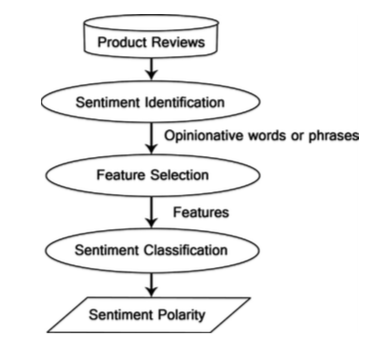
\includegraphics[scale=0.45]{./images/sa_process}
	\caption{Sentiment analysis process on product reviews}
\end{figure}
\end{columns}
\end{frame}

%Sentiment analysis: a classification problem
\begin{frame}
\frametitle{Sentiment analysis: a classification problem}
\begin{figure}
	\centering
	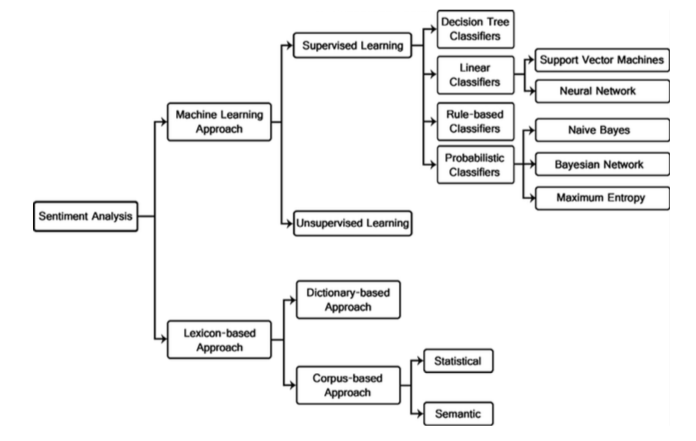
\includegraphics[scale=0.4]{./images/sentiment_classification}
	\caption{Sentiment classification techniques}
\end{figure}
\end{frame}

%Emotion Detection (ED)
\begin{frame}
\frametitle{Emotion Detection (ED)}
\begin{definition}
Emotion detection is the process of identifying human emotions.
\end{definition}
\begin{block}{Remark}
Emotion Detection (ED) is a SA task.
\end{block}
SA  $\rightarrow$ detects positive or negative feeling from text.\\
ED  $\rightarrow$ detects various emotions.\\
\end{frame}

%Emotion Detection: Why
\begin{frame}
\frametitle{Emotion Detection: Why}
Emotion detection has useful applications, such as: 
\begin{itemize}
\item Measure citizens happiness
\item Pervasive computing
\item Understanding customers
\end{itemize}
\begin{block}{Our goal}
Unravel emotion patterns in the playlists
\end{block}
\end{frame}

%Emotion Detection: Challenges
\begin{frame}
\frametitle{Emotion Detection: Challenges}
(Some of the) Biggest challenges in ED:
\begin{itemize}
\item Context-dependence of emotions $\Rightarrow $ people use different emotion regulation strategies in different social contexts
\item Word-sense disambiguation $\Rightarrow $ identifying which sense of a word (i.e. meaning) is used in a sentence, when the word has multiple meanings
\item Co-reference resolution $\Rightarrow $ pronouns and other referring expressions must be connected to the right individuals
\item Lack of labelled emotion database
\end{itemize}
\end{frame}

\section{Main methods}
%Methods for Emotion Detection
\begin{frame}{Methods for Emotion Detection}
Methods used for text based emotion detection are: 
\begin{enumerate}
\item Keyword Spotting
\item Lexical Affinity
\item Learning-based 
\item Hybrid
\end{enumerate}
\end{frame}

%Keyword Spotting method
\begin{frame}{1. Keyword spotting method}
\begin{columns}
\column{0.5\textwidth}
Finding occurrences of keywords from a given set. These words are classified into categories such as disgusted, sad, happy, angry, etc. 
\column{0.5\textwidth}
\begin{figure}
	\centering
	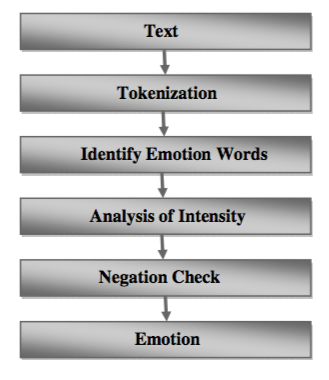
\includegraphics[scale=0.45]{./images/keyword_spotting}
	\caption{Keywork Spotting Technique}
\end{figure}
\end{columns}
\end{frame}

%Lexical Affinity method
\begin{frame}{2. Lexical Affinity method}
Is an extension of keyword spotting technique: apart from picking up emotional keywords it assigns  probabilistic `affinity' for a particular emotion to arbitrary words.\\
Disadvantages: 
\begin{itemize}
\item assigned probabilities are biased toward corpus-specific genre of texts
\item it misses out emotion content that resides deeper than the word-level
\end{itemize}
\begin{example}
``I avoided an accident"\\
``I met my girlfriend by accident"
\end{example}
\end{frame}

%Learning-based Method
\begin{frame}{3. Learning-based methods}
\begin{block}{Remark}
FROM determine emotions TO classify the input texts into different emotions
\end{block}
Learning based methods try to detect emotions based on a previously trained classifier, which apply various theories of machine learning such as SVM.
\end{frame}

%Limitations
\begin{frame}{Limitations}
\begin{columns}
\column{0.5\textwidth}
Major limitations:
\begin{itemize}
\item Ambiguity in keyword definition
\item Incapability of recognizing sentences without keywords
\item Lack of linguistic information
\item Difficulties in determining emotion indicators
\end{itemize}
\column{0.5\textwidth}
\begin{example}
``I passed my qualify exam today"\\
``Hooray! I passed my qualify exam today"
\end{example}
\begin{example}
``He laughed at me"\\
``I laughed at him"
\end{example}
\end{columns}
\end{frame}



\section{Emotion Classification}

% Feature selection
\begin{frame}{Feature Selection}
Which textual features are we interested in?
\begin{itemize}
\item Terms presence and frequency
\item Adjectives
\item Opinion Words and Phrases
\item Negation expressions
\end{itemize}
\end{frame}

% Feature selection methods (Davvero utile?)
\iffalse
\begin{frame}{Feature Selection Methods}
\begin{itemize}
\item Strings
\begin{itemize}
\item Phrases representing emotional patterns
\end{itemize}
\item Bag of Words (BoW)
\begin{itemize}
\item Sort of keywords list
\item Make the classification process simpler
\end{itemize}
\end{itemize}
\end{frame}
\fi

% Classification Levels I
\begin{frame}{Classification Levels (I)}
Three possible classification levels:
\begin{itemize}
\item Document Level 
\begin{itemize}
\item The whole document is the classification unit
\end{itemize}
\item Sentence Level
\begin{itemize}
\item Sentences are the basic classification units
\end{itemize}
\item Aspect Level
\begin{itemize}
\item Classify sentiments with respect to entities and their aspects
\end{itemize}
\end{itemize}
\end{frame}

% Classification Levels II
\begin{frame}{Classification Levels (II)}
\textbf{Document level} classification suits our problem
\begin{itemize}
\item We will analyze lyrics
\item Lyrics are (usually) small documents focused on a single topic
\item We can treat lyrics as our classification unit
\end{itemize}
\end{frame}


%How many sentiments
\begin{frame}{How many sentiments?}
Human can have an enormous range of different sentiments and moods
\begin{itemize}
\item Anger
\item Sadness
\item Happiness
\item Surprise
\item Fear
\item Disgust
\item ...
Which of them may be related to lyrics?
\end{itemize}
\end{frame}

%How to label them?
\begin{frame}{How to label them?}
We may label lyrics to be exactly related to one mood/sentiment.
\begin{itemize}
\item Is it accurate?
\item Is it possible that one song express more sentiments? $\rightarrow$ Sliders approach
\end{itemize}
\end{frame}

%The sliders approach
\begin{frame}{The ``sliders" approach}
Assigning a value to each possible sentiment may be more flexible.
\begin{figure}
	\centering
	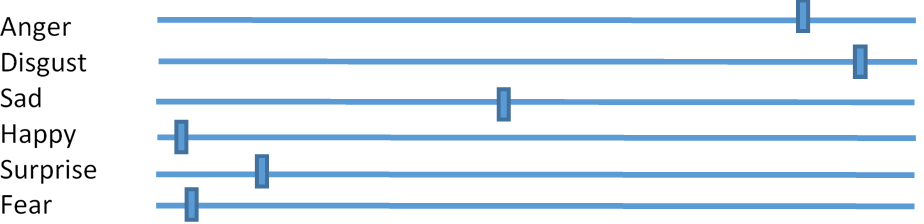
\includegraphics[scale=0.35]{./images/emotion_labeling_sliders}
\end{figure}
Do we really need this level of flexibility in our application?
\end{frame}

\begin{frame}{Emotion Dimensions}
\begin{columns}
\column{0.5\textwidth}
Current systems tends to classify emotions according to two dimensions
\begin{itemize}
\item Arousal
\item Valence
\end{itemize}
\column{0.5\textwidth}
\begin{figure}
	\centering
	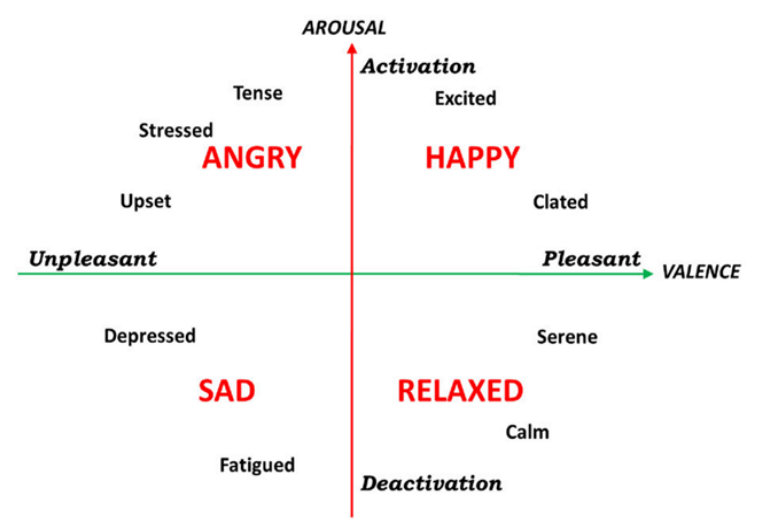
\includegraphics[scale=0.3]{./images/emotion-dimensions}
\end{figure}
\end{columns}
\end{frame}

% Conclusion

\section{Conclusion}

\begin{frame}{Datasets}
There are very few datasets which could suits our case
\begin{itemize}
\item MoodyLyrics is the most relevant example of that\footnote{Look at the references for the releated article}
\begin{itemize}
\item It uses only 4 emotions (Happy, Sad, Angry and Relaxed)
\item Is it enough?
\end{itemize}
\end{itemize}
\end{frame}


\begin{frame}{What we learnt}
\begin{itemize}
\item Defining the number of moods we want to consider is not an easy task but probably we don't
	need many of them because our analysis domain is restricted to songs
\item The "sliders" approach is too general. Songs are usually linked with a single sentiment
\item We should not overcomplicate our emotion range
\item Using already annotated lyrics datasets could he helpful
\end{itemize}
\end{frame}

%References

\section{References}
\begin{frame}{References}
\setbeamertemplate{bibliography item}[triangle]
 \begin{thebibliography}{99} % Beamer does not support BibTeX so references must be nserted manually as below
\bibitem[Microsoft, 2015]{p1} Microsoft Developer Blog (2015)
\newblock Emotion detection and recognition from text using Deep Learning
\newblock \href{https://www.microsoft.com/developerblog/2015/11/29/emotion-detection-and-recognition-from-text-using-deep-learning/}{link}

\bibitem[Survey 2014]{p2} Walaa Medhat, Ahmed Hassan, and Hoda Korashy (2014)
\newblock Sentiment Analysis Algorithms and Applications: A Survey.
\newblock \emph{Ain Shams Engineering Journal}

\bibitem[Ed from text]{p3} Shiv Naresh Shivhare1 and Prof. Saritha Khethawat (2012)
\newblock Emotion Detection From Text

\end{thebibliography}

\end{frame}

\begin{frame}{References}
\setbeamertemplate{bibliography item}[triangle]
 \begin{thebibliography}{99} % Beamer does not support BibTeX so references must be nserted manually as below

\bibitem{p4}Hu, Xiao and Downie, J. Stephen and Ehmann, Andreas F. (2009)
\newblock Lyric Text Mining in Music Mood Classification.
\newblock \emph{Society for Music Information Retrieval}

\bibitem{p5}Çano, Erion and Morisio, Maurizio  (2017)
\newblock  MoodyLyrics: A Sentiment Annotated Lyrics Dataset.
\newblock \emph{International Conference on Intelligent Systems, Metaheuristics \& Swarm Intelligence, Hong Kong, March, 2017}

\end{thebibliography}

\end{frame}
%---------------------------------------------------------

\end{document}
